\documentclass[UTF8]{ctexart}
\CTEXsetup[format={\Large\bfseries}]{section}%默认一级标题居左
\usepackage{geometry}
\geometry{left=2.5cm,right=2.5cm,top=2.5cm,bottom=2.5cm} %页边距
\usepackage{graphicx}%图形
\usepackage{fancyhdr}%页眉页脚
\pagestyle{fancy}	%启用fancy风格设置
\lhead{}
\chead{}
\rhead{\bfseries\textsl{\today}  }
\lfoot{}
\cfoot{\thepage}
\rfoot{}
%\renewcommand{\headrulewidth}{0.6pt}    %单线页眉的设置 
\renewcommand{\footrulewidth}{0.4pt}     %单线页脚的设置 
%-----------双线页眉的设置  
\makeatletter % 进入“内部命令模式”(允许使用 @ 符号的 LaTeX 内部变量)
\def\headrule{{\if@fancyplain\let\headrulewidth\plainheadrulewidth\fi%
		\hrule\@height 1.0pt \@width\headwidth\vskip1pt%上面线为1pt粗  
		\hrule\@height 0.5pt\@width\headwidth  %下面0.5pt粗            
		\vskip-2\headrulewidth\vskip-4pt}      %两条线的距离1pt        
		  \vspace{3mm}}     %双线与下面正文之间的垂直间距 
\makeatother    % 退出“内部命令模式”
%------------双线页眉的设置            
% \usepackage{booktabs}
% \usepackage{subfigure}
\usepackage{setspace}
\usepackage{array}%需要该宏包
\usepackage{diagbox} % 加载宏包
\usepackage{multirow}
\usepackage{textcomp}
\usepackage{indentfirst}%首行缩进宏包
\usepackage{setspace}
\usepackage{amssymb}
\usepackage{amsmath} %数学公式
\usepackage{listings} %代码块
\usepackage{xcolor} %设置颜色,例如基础高亮
\usepackage[colorlinks=true,pdfborder={0 0 0},
    linkcolor=red,     % 内部链接(如目录→章节)的文字颜色
    citecolor=green,    % 引用(如\cite)的文字颜色
    urlcolor=blue,      % 网址的文字颜色
]{hyperref} %超链接
\usepackage{attachfile2}
\lstset{
    language=[LaTeX]TeX, % 指定语言为 LaTeX
    basicstyle=\ttfamily\small, % 基本字体设置
    % keywordstyle=\color{blue}, % 关键字颜色
    commentstyle=\color{gray}, % 注释颜色
    stringstyle=\color{red}, % 字符串颜色
    showstringspaces=false, % 不显示字符串中的空格标记
    numbers=left, % 行号位置
    numberstyle=\tiny\color{gray}, % 行号样式
    frame=single, % 边框样式
    breaklines=true, % 自动换行
    escapeinside={\%*}{*)} % 允许在代码中插入 LaTeX 命令
}


\title{{\heiti  第一周实验:Git、LaTeX }\vspace{-2em}}
\date{}
\begin{document}
\thispagestyle{empty}  %用于设置 “当前页” 的页眉页脚风格:
\begin{figure}[tph!] %封面标题
	\centering
	
\includegraphics[width=0.7\linewidth]{figure/2}
	
\end{figure}

\begin{center}% % 内容居中环境(所有内部内容均居中对齐)
	\quad \\ %插入一个小空格
	\quad \\
	\quad \\
	\quad \\
	% \quad \\
	% \quad \\
	\heiti \fontsize{30}{17} \quad \quad 第\quad 一\quad 周\quad \quad \quad 
	\vskip 0.5cm
	\songti \zihao{2} 实\quad 验\quad 报\quad 告%在此打印论文题目,二号黑体	
\end{center}
\vskip 1cm

\begin{quotation}
	\songti \fontsize{20}{20}
	\doublespacing
	\par\setlength\parindent{12em}
	\qquad
\begin{center}
		{\Large 学\hspace{0.88cm} 院:\underline{\hbox to 58mm{信息科学与工程学部\hfill}}}
		\vskip 0.3cm	
		{\Large 班\hspace{0.88cm} 号:\underline{\hbox to 58mm{计科一班\hfill}}}
		\vskip 0.3cm
		{\Large 姓\hspace{0.88cm} 名:\underline{\hbox to 58mm{顾晓宁\hfill}}}
		\vskip 0.3cm	
		{\Large 学\hspace{0.88cm} 号:\underline{\hbox to 58mm{24020007036\hfill}}}
		\vskip 0.3cm	
		{\Large 实验编号:\underline{\hbox to 58mm{第一周实验报告\hfill}}}
		\vskip 0.3cm	
		{\Large 指导教师:\underline{\hbox to 58mm{周小伟\hfill}}}
	\end{center}
	% \vskip 3cm
	% \begin{flushright}% 日期右对齐
	% 	% 2019\;年\;5\;月\;14\;日
	% 	\today
	% \end{flushright}
	
\end{quotation}
\newpage
%\thispagestyle{empty}
\tableofcontents % 自动生成目录(基于后续的 \section、\subsection 等章节命令)
\newpage
\maketitle	
\thispagestyle{fancy}	
\section{实验目的}
\textbf{练习使用Git进行版本控制,掌握LaTeX的基本使用方法}

\section{练习内容与结果}
\textbf{注意,以下内容均为练习实例,一般不含解释;语法等具体知识点看参照文末相关资料}\\
\textbf{同时该练习实例较为简陋,一般用于根据模板编写LaTex,倘若对格式有更高或者自定义需求,建议系统、完整地参阅文档学习}

\subsection{LaTex 练习实例}

\subsubsection{LaTex的基本区域、以及最基础的框架是?}
在LaTex中,文档的基本结构包括导言区和正文区。导言区用于设置文档的类型、加载宏包和定义自定义命令,而正文区则包含实际的内容。
\begin{lstlisting}[language=Tex]
\documentclass[UTF8]{ctexart}
\title{title}
\author{author}
\date{\today}
% above is preamble that sets up the document
\begin{document}
\maketitle
This is the content of the document.
\end{document}
\end{lstlisting}

\subsubsection{常用的设置文字的设置有?}
\begin{lstlisting}[language=Tex]
\textbf{Bold text}
\textit{Italic text} 
\underline{Underlined text} 
\end{lstlisting}
展示:\\
\textbf{Bold text} \\
\textit{Italic text} \\
\underline{Underlined text}

\subsubsection{常用的章节命令有?}
part$>$chapter$>$section$>$subsection$>$subsubsection\\
\begin{lstlisting}[language=TeX]
\section{Level 1 Heading}
\subsection{Level 2 Heading}
\subsubsection{Level 3 Heading}
\chapter{Chapter Heading} % Only in book/report class
\part{Part Heading} % Only in book/report class
\end{lstlisting}

\subsubsection{LaTex特殊符号有?且如何显示在文本中?}
特殊字符如下:\\
\begin{table}[htbp]
\begin{tabular}{ll}
\verb|%| & 注释符号 \\
\verb|&| & 表格对齐符号 \\
\verb|$| & 数学模式标记 \\
\verb|~| & 非断行空格 \\
\verb|^| 和 \verb|_| & 上下角标 \\
\verb|{| 和 \verb|}| & 分组符号 \\
\verb|#| & 宏定义符号 \\
\verb|\| & 转义符号 \\
\verb|\\| & 换行符 \\
\end{tabular}
\centering
\caption{特殊字符}
\label{specialChar}
\end{table}
\begin{lstlisting}[language=Tex]
\verb|char|
\end{lstlisting}
该命令逐字打印,用于显示LaTeX代码、特殊字符等,而不被LaTeX解释。\\
\verb'|'是分隔符,可以用任何字符,如'(但不能是要显示的文本中包含的字符)\\
分隔符内的所有内容都会原样输出。\\
也可以使用\verb|\texttt{}|,同样可以打印特殊字符。\\

\subsubsection{如何换行、换段、换页、首行缩进?}
\begin{lstlisting}[language=Tex]
\\ % to newline
\newline \linebreak % alse to newline
\par % to new paragraph
\newpage % to new page
\setlength{\parindent}{length} %first line indentation
\noindent % to set no indentation in a line
\end{lstlisting}
展示:
% 设置首行缩进
\setlength{\parindent}{2em} % 2字符缩进

这是第一段文本。\par % 使用 \par 分段
这是第二段文本,通过 \verb|\par| 命令分隔。

这是第三段文本,使用空行分段(效果与 \verb|\par| 相同)。

这是第四段文本。

\newpage % 分页命令

这是新的一页内容。分页后从这里开始。

% 改变缩进设置
\setlength{\parindent}{0pt} % 取消缩进
这段没有首行缩进。

\setlength{\parindent}{4em} % 4字符缩进
这段有更大的缩进。\\
\setlength{\parindent}{0pt}
此外,常用的缩进命令有:\\
\begin{lstlisting}
\hspace{1cm} % 1cm Horizontal indentation
\quad % 1 space,whitch equal to 1em
\qquad % 2 space
\vspace{10pt} downward vertical indentation
\vspace{-10pt} above vertical indentation
\end{lstlisting}

\subsubsection{LaTex的box如何使用?}

\begin{lstlisting}
\hbox{text}
\hbox to width{text}
\vbox{text}
\makebox[width][align]{text} % The most commonly used
\framebox[width][align]{text}
% align : l\c\r\s , s:scatter
\end{lstlisting}
\begin{verbatim}
\parbox[基线对齐位置tcb][height][内部对齐]{宽度}{内容}
\end{verbatim}
展示,用四个makebox展示左中右分散对齐,1个framebox,1个parbox:\\
\makebox[3cm][l]{左对齐} \\  % 左对齐
\makebox[3cm][c]{居中}     \\% 居中对齐
\makebox[3cm][r]{右对齐}  \\ % 右对齐
\makebox[3cm][s]{分散对齐} \\% 分散对齐
\framebox[3cm][c]{带框盒子}\\
% 基本语法
% \parbox[位置][高度][内部位置]{宽度}{内容}
\parbox{5cm}{这是一个较长的段落文本,会在指定的5厘米宽度内自动换行。}\\


\subsubsection{如何插入图片?}
\begin{lstlisting}
\usepackage{graphicx} % in preamble
% then in document;and Omit some content
\begin{figure}[htbp]
	\centering
	\includegraphics[width=0.5\textwidth]{path/to/image}
	\caption{Caption text}
	\label{fig:label}
\end{figure}
\end{lstlisting}
展示:
\begin{figure}[htbp]
	\centering
	
\includegraphics[width=0.5\textwidth]{figure/2.1.4}
	\caption{图片示例}
	\label{figure2.1.4}
\end{figure}

\subsubsection{如何插入列表?}
列表有无序和有序之分
\begin{lstlisting}
% Unordered list
\begin{itemize}
	\item First item
	\item Second item
	\item Third item
\end{itemize}
% Ordered list
\begin{enumerate}
	\item First item
	\item Second item
	\item Third item
\end{enumerate}
\end{lstlisting}
展示:\\
无序
\begin{itemize}
	\item First item
	\item Second item
	\item Third item
\end{itemize}
有序
\begin{enumerate}
	\item First item
	\item Second item
	\item Third item
\end{enumerate}

\subsubsection{如何插入数学公式?}
\begin{lstlisting}
$E=mc^2$ % Inline math mode

\begin{equation}
E=mc^2 % Display math mode with number
\end{equation}

\[
a^2 + b^2 = c^2 % Display math mode without number
\]
% or use $$ math mode $$

% if too long
\begin{split}
a & = b + c + d + e + f + g + h + i + j + k + l + m + n + o + p \\
  & \quad + q + r + s + t + u + v + w + x + y + z
\end{split}

% discuss case by case
f(x)=
\begin{cases}
1, & \text{if } x > 0 \\
0, & \text{if } x = 0 \\
-1, & \text{if } x < 0
\end{cases}
\end{lstlisting}
展示:\\
\text{单行公式}\\
$E=mc^2$\\
单行带编号\\
\begin{equation}
a^2 + b^2 = c^2
\end{equation}
单行不带编号\\
\[
a^2 + b^2 = c^2
\]
由于split和cases需要在数学环境中使用,此处选择将其包含在equation环境中。\\
多行\\
\begin{equation}
\begin{split}
a &= b + c + d + e + f + g + h + i + j + k + l + m + n + o + p \\
  &\quad + q + r + s + t + u + v + w + x + y + z
\end{split}
\end{equation}

根据条件分类\\
\begin{equation}
f(x)=
\begin{cases}
1, & \text{if } x > 0 \\
0, & \text{if } x = 0 \\
-1, & \text{if } x < 0
\end{cases}	
\end{equation}

\subsubsection{如何插入表格?}
\begin{lstlisting}
\begin{table}
\centering
\begin{tabular}{|c|c|c|}
\hline
Header 1 & Header 2 & Header 3 \\
\hline
Cell 1 & Cell 2 & Cell 3 \\
\hline
Cell 4 & Cell 5 & Cell 6 \\
\hline
\end{tabular}
\caption{Sample Table}
\label{tab:sample}
\end{table}
\end{lstlisting}
展示:\\
\begin{table}[htbp]
\centering
\begin{tabular}{|c|c|c|}
\hline
Header 1 & Header 2 & Header 3 \\
\hline
Cell 1 & Cell 2 & Cell 3 \\
\hline
Cell 4 & Cell 5 & Cell 6 \\
\hline
\end{tabular}
\caption{Sample Table}
\label{tabel2.1.7}
\end{table}

\subsubsection{如何引用参考文献?}
\textbf{注意,你通常需要两次编译。LaTeX 中,交叉引用(如公式、章节编号)、参考文献的链接信息,需要在第一次编译时记录位置,第二次编译时才能正确插入。}\\

简单的用法:\\
\begin{lstlisting}
% references
\begin{thebibliography} {}
\bibitem{label 1} ...content...
\bibitem{label 2} ...content...
\end{thebibliography}
% how to cite them
\cite{label}
\end{lstlisting}
展示:\\
\begin{lstlisting}[language=Tex]
\section{references}
\begin{thebibliography}{9} 
	\bibitem{bib:one} ...content...
\end{thebibliography}
% use \cite{bib:one} to cite it
\end{lstlisting}
常用用法:\\
\begin{lstlisting}
\cite{label} % to cite 
\bibliographystyle{unsrt} %in main body
\bibliography{bibFileName} % add references
\end{lstlisting}
展示:\\
根据爱因斯坦的相对论\cite{einstein1905},时间和空间是相对的。\\
多项研究表明...\cite{einstein1905, knuth1984, lamport1985},这些工作对科学和出版领域产生了深远影响。\\

\subsubsection{除文献外,如何引用表格、图片等内容?}
\begin{lstlisting}
\usepackage{hyperref} % preamble
% after setting label
\autoref{label}
\end{lstlisting}
展示:\\
展示Latex的特殊字符的表格是:\autoref{specialChar}

\subsubsection{如何插入代码?}
\textbf{注意,也包括LaTex代码;对于参数也可以额外设置;}
\begin{verbatim}
\usepackage{listings} % centeral package
\usepackage{xcolor} % optional,to set color
\begin{lstlisting}[language=Python]
...
\end{lstlisting}
% follow is style-settings
\lstset{
    language=[LaTeX]TeX, % 指定语言为 LaTeX
    basicstyle=\ttfamily\small, % 基本字体设置
    keywordstyle=\color{blue}, % 关键字颜色
    commentstyle=\color{gray}, % 注释颜色
    stringstyle=\color{red}, % 字符串颜色
    showstringspaces=false, % 不显示字符串中的空格标记
    numbers=left, % 行号位置
    numberstyle=\tiny\color{gray}, % 行号样式
    frame=single, % 边框样式
    breaklines=true, % 自动换行
    escapeinside={\%*}{*)} % 允许在代码中插入 LaTeX 命令
}
\end{verbatim}
可以直接导入外部的代码文件:
\begin{verbatim}
\lstinputlisting[language=,numbers=]{demo.py}
\end{verbatim}
展示:\\
\lstinputlisting[language=Python,numbers=left]{demo.py}
也可以使用下面这个命令,来导入代码:\\
\begin{lstlisting}
\begin{verbatim}
...
\end{verbatim}
\end{lstlisting}

\subsubsection{如何插入链接?}
\begin{lstlisting}
\usepackage{hyperref}
\href{url}{description}
\url{url} % directly displat this url
\href{mailto:email_address}{text} % add email address
\end{lstlisting}
展示,其中邮箱example@outlook.com是任意设置的:\\
\href{https://www.latex-project.org/}{LaTex官网}\\
\url{https://www.latex-project.org/}\\
\textbf{注意:部分游览器无法解析mailto协议,导致将其视为网址的一部分}\\
\href{mailto:sufferingwish@outlook}{MyEmail}\\
\textit{值得一提的是pdfborder可以被打印出来,可以手动将其取消,示例如下:}
\begin{lstlisting}
\usepackage[colorlinks=true,pdfborder={0 0 0},
    linkcolor=red,     
    citecolor=green,    
    urlcolor=blue,   
]{hyperref} 
\end{lstlisting}

\subsubsection{LaTex模板和页边距等如何设置?}
具体可见本目录下template.tex文件
%\autoref{}

\subsection{Git 练习实例}
\subsubsection{从历史中删除文件}
\textbf{使用 Git 时的一个常见错误是提交本不应该由 Git 管理的大文件,或是将含有敏感信息的文件提交给 Git 。尝试向仓库中添加一个文件并添加提交信息,然后将其从历史中删除}
\\
答案解析中提供了一种强大且危险的命令,来删除所有历史中$my_password$文件。
该操作会改变哈希值,建议仅在本地使用。
\\
\begin{lstlisting}
 git filter-branch --force --index-filter\
 'git rm --cached --ignore-unmatch ./my_password' \
 --prune-empty --tag-name-filter cat -- --all
\end{lstlisting}
不过也有其他方法可用,适用于本地且该危险提交发生不久,优点是命令简单,例如:\\
\begin{lstlisting}
git reset --hard <commit_hash>
\end{lstlisting}
\begin{figure}[htbp]
\centering
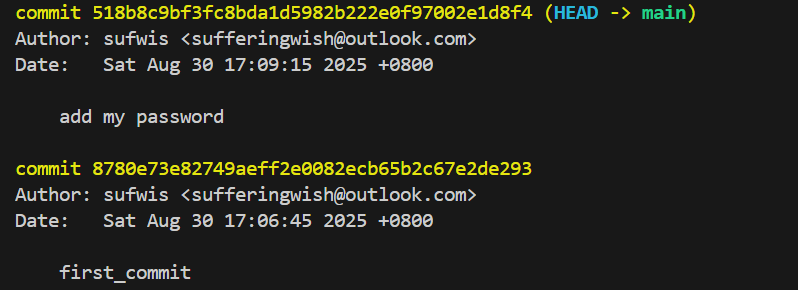
\includegraphics[width=0.7\linewidth]{./figure/add_password}
\caption{添加密码文件}
\end{figure}
\begin{figure}[htbp]
\centering
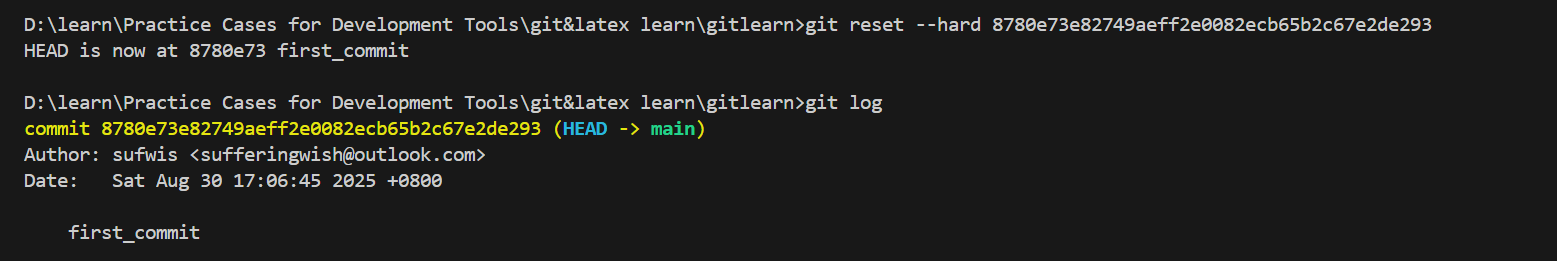
\includegraphics[width=0.7\linewidth]{./figure/back_firstcommit}
\caption{执行回滚}
\end{figure}
\textbf{回滚后,如图可见log中并无第二次commit}\\
\begin{figure}[htbp]
\centering
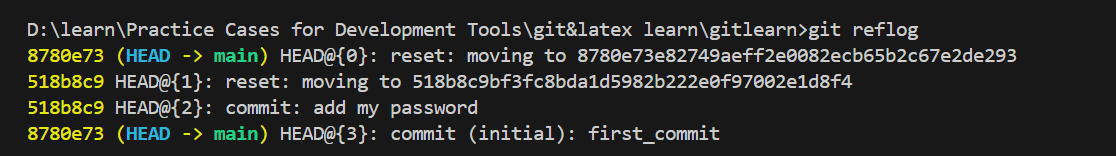
\includegraphics[width=0.7\linewidth]{./figure/look_fromgitreflog}
\caption{通过git reflog 查看HEAD移动记录}
\end{figure}
\\\textbf{此处,虽然git保留了添加密码的移动记录,但是并不会被push到远端仓库。}
git reflog能够查看几乎所有移动过的快照,同时具有本地性和时效性——一段时间后会自动清理。
配合回滚操作,能够做到恢复大部分文件的效果,通常应用于误删。
\\

\subsubsection{从 GitHub 上克隆某个仓库,修改一些文件。当您使用 git stash 会发生什么?当您执行 git log --all --oneline 时会显示什么?通过 git stash pop 命令来撤销 git stash 操作,什么时候会用到这一技巧?}
git stash: 暂存工作区和暂存区\\
git log --all --oneline: 显示所有本地和远端分支信息,且以oneline即一行的形式,仅保留哈希值、提交信息、引用信息\\
git stash pop: 恢复最近的一次git stash保存的修改,并将该 stash 从 stash 列表中移除。通常用于:
\begin{center}
	中断当前任务,处理紧急任务;\\
	尝试不同的解决方案;\\
	合并分支前暂存修改;
\end{center}
\begin{figure}[htbp]
\centering
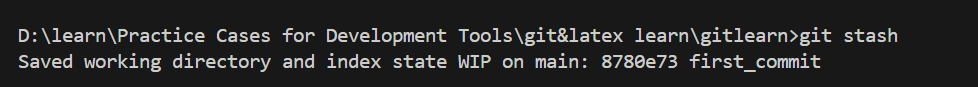
\includegraphics[width=0.7\linewidth]{./figure/stash.png}
\caption{使用git stash}
\end{figure}
\begin{figure}[htbp]
\centering
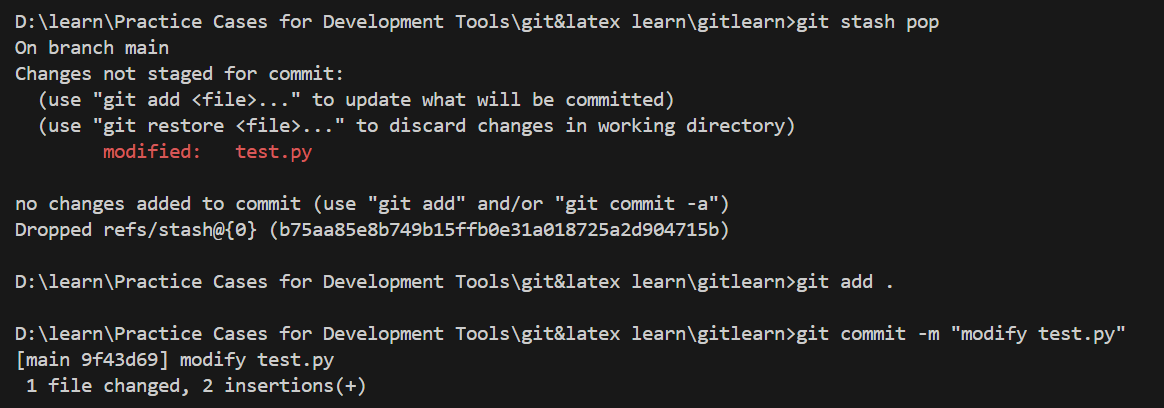
\includegraphics[width=0.7\linewidth]{./figure/stash_pop.png}
\caption{使用git stash pop}
\end{figure}
当我修改test.py后,并未暂存。而是直接使用git stash。
之后新建分支,做一次提交后,签出到main分支,使用git stash pop。
此时,test.py文件恢复到使用stash暂存时的状态。

\subsubsection{如何在git中创建别名?}
\begin{enumerate}
	\item git config --global alias.<缩写> <原命令>
	\item 设置局部别名(仅对当前仓库有效):去掉 --global 参数即可
	\item 直接编辑配置文件.gitconfig
\end{enumerate}
\begin{figure}[htbp]
\centering
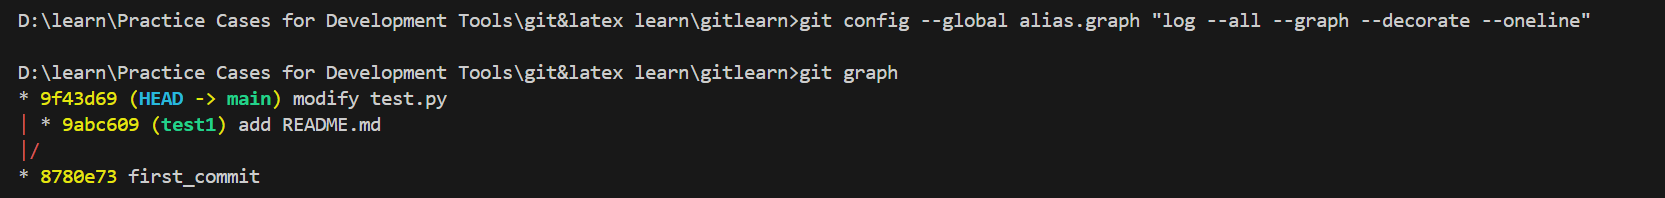
\includegraphics[width=\linewidth]{./figure/config.png}
\caption{使用git config --global alias.缩写 原命令}
\end{figure}
结果如图\\

\subsubsection{git如何忽略文件?}
\textbf{通常,建议常见一个.gitignore文件,在其中写入要删除的文件即可。可以使用**匹配任意目录。}

\subsubsection{git使用流程?}
方法一:\\
从本地,简述为:init 初始化 add. commit 提交,remote add origin,push -u origin main 推送\\
方法二:\\
从远端,git clone 下分支;\\
\\
\textit{git常用指令可见附件}\\
\attachfile[description=git指令]{./gitlearn/Git.txt}{双击}\\
如果浏览器无法解析,可见./gitlearn/Git.txt\\
\section{实验感悟}
\qquad\textbf{从LaTex的学习中可以了解到,只有亲自动手练习才是增进熟练度最合适的方式。}
LaTex能够精确控制文档格式,支持数学符号和公式,常用于论文设置。尽管仅仅只是简单地学习其语法,
以及基础的使用方法,也能感受到它的强大。
\textbf{无疑,LaTex是值得推荐的。}
对于有更高需求的使用者,深入学习LaTex也是必要的。\\

\qquad\textbf{Git不必多言,最常用且最受欢迎的版本控制工具之一。}
不管是用于本地管理,还是远端与他人协同工作,git 常常能够提供有力的帮助。
如果只是处于使用的考量,学习使用git指令,或者安装对应插件是不错的选择。
同时也推荐了解其工作原理,这会对理解git的回滚很有帮助.倘若时间富余,也可深入研究。

\section{参考文献示例,仅用于演示}
\bibliographystyle{unsrt}
\bibliography{references}

\section{个人github账号}
\href{https://github.com/sufwis}{个人github账号}\\
\href{https://github.com/sufwis/development-tools-learn.git}{对应仓库}

\section{相关资料}
\href{https://gitcode.com/Premium-Resources/7dbf2.git}{LaTex模板改自此处}\\
\href{https://oi-wiki.org/tools/latex/}{LaTex参考资料}\\
\href{https://www.latex-project.org/}{LaTex官网}\\
\href{https://missing-semester-cn.github.io/}{git相关参考资料}
\end{document}